\documentclass{gradpaper}


\university{Universidade Federal de Pernambuco}
\institute{Centro de Informática}
\address{Recife}
\degree{Graduate}
\majorfield{Computer Engineering}
\title{Improvements in Speaker Verification using Fractional Covariance Matrix}
%\date{TODO colocar a data da defesa}
\author{Eduardo Martins Barros de Albuquerque Tenório}
\adviser{Tsang Ing Ren}
\advisertitle{Dr.}
\reviser{George Darmiton da Cunha Cavalcanti}
\revisertitle{Dr.}


\begin{document}

% Frontmatter

\frontpage
\presentationpage
\signatures

\acknowledgements{I am thankful to my parents, for the support and patience
during this long graduation,
\\To my adviser, Tsang Ing Ren, for the guidance,
\\To the colleagues Hector Pinheiro and Sérgio Renan Vieira, for helping me to understand the
GMM.
}

\epigraph{Live long and prosper}{Vulcan salute}

\abstract
abstract
\begin{keywords}
keywords
\end{keywords}

% TODO verificar se as listas possuem # de paginas impar ou par
\afterpage{\frontmatterblankpage}
\listoffigures
\listoftables
\tableofcontents


% Mainmatter

\clearpage
\setcounter{page}{1}
\section{Extração de Características}
\label{sec:feature-extraction}

\contentscurrent

\begin{frame}
\frametitle{Características Ideais}
\begin{itemize}
    \item Natural e frequente na fala
    \pause
    \item Facilmente mensurável
    \pause
    \item $\uparrow$ variação inter-locutor e $\downarrow$ variação intra-locutor
    \pause
    \item Constante no tempo e não afetável pela saúde
    \pause
    \item Robusta a ruído razoável e a transmissão
    \pause
    \item Difícil de ser produzido artificialmente
    \pause
    \item Não ser facilmente modificável pelo locutor
\end{itemize}
\end{frame}

\subsection{MFCC}

\begin{frame}
\frametitle{Mel-Frequency Cepstrum Coefficients}
\begin{description}
    \item Simula a função da \textbf{cóclea}
    \pause
    \item[Escala Mel] Logaritmica
    \pause
    \begin{itemize}
        \item $f_{mel} = 2595 \log_{10}(1 + \frac{f}{700})$
        \pause
    \end{itemize}
\end{description}

\begin{figure}[ht]
    \centering
    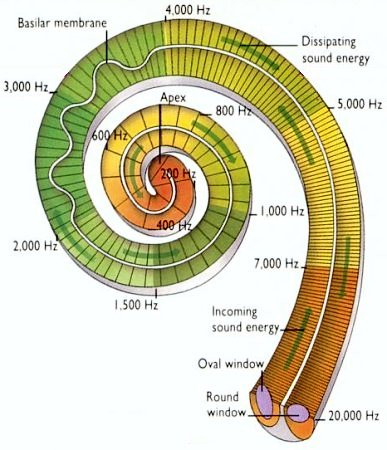
\includegraphics[width=0.35\textwidth]{cochlea}
\end{figure}
\end{frame}

\subsection{MFCC - Extração}

\begin{frame}
\frametitle{MFCC - Extração}
\begin{figure}[ht]
    \centering
    
\includegraphics[width=0.75\textwidth]{mfcc-flow}
\end{figure}
\pause

\begin{description}
    \item[Pré-ênfase] \textbf{Realça} as altas frequências (opcional)
    \pause
    \begin{itemize}
        \item $s_{emph}[n] = s[n] - \alpha \cdot s[n - 1]$
        \pause
        \item $\alpha \in [0.95, 0.98]$
        \pause
    \end{itemize}
\end{description}
\begin{figure}[ht]
    \centering
    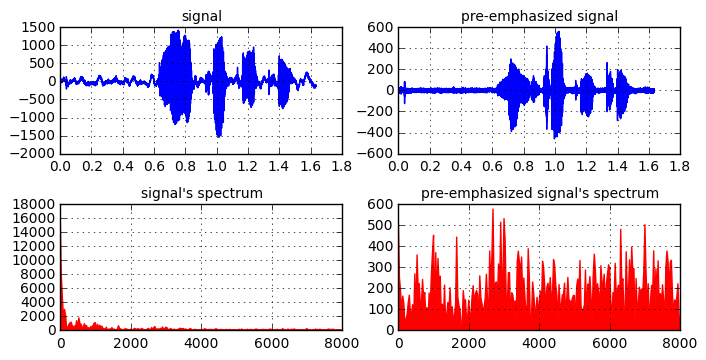
\includegraphics[width=0.75\textwidth]{preemphasis}
\end{figure}
\end{frame}

\subsection{MFCC - Extração}

\begin{frame}
\frametitle{MFCC - Extração}
\begin{figure}[ht]
    \centering
    
\includegraphics[width=0.75\textwidth]{mfcc-flow}
\end{figure}
\pause

\begin{description}
    \item[Janelamento] Divide o sinal em janelas \textbf{superpostas}
    \pause
    \begin{itemize}
        \item Largura de 20 milissegundos
        \pause
        \item Deslocamento de 10 milissegundos
        \pause
    \end{itemize}
\end{description}
\begin{figure}[ht]
    \centering
    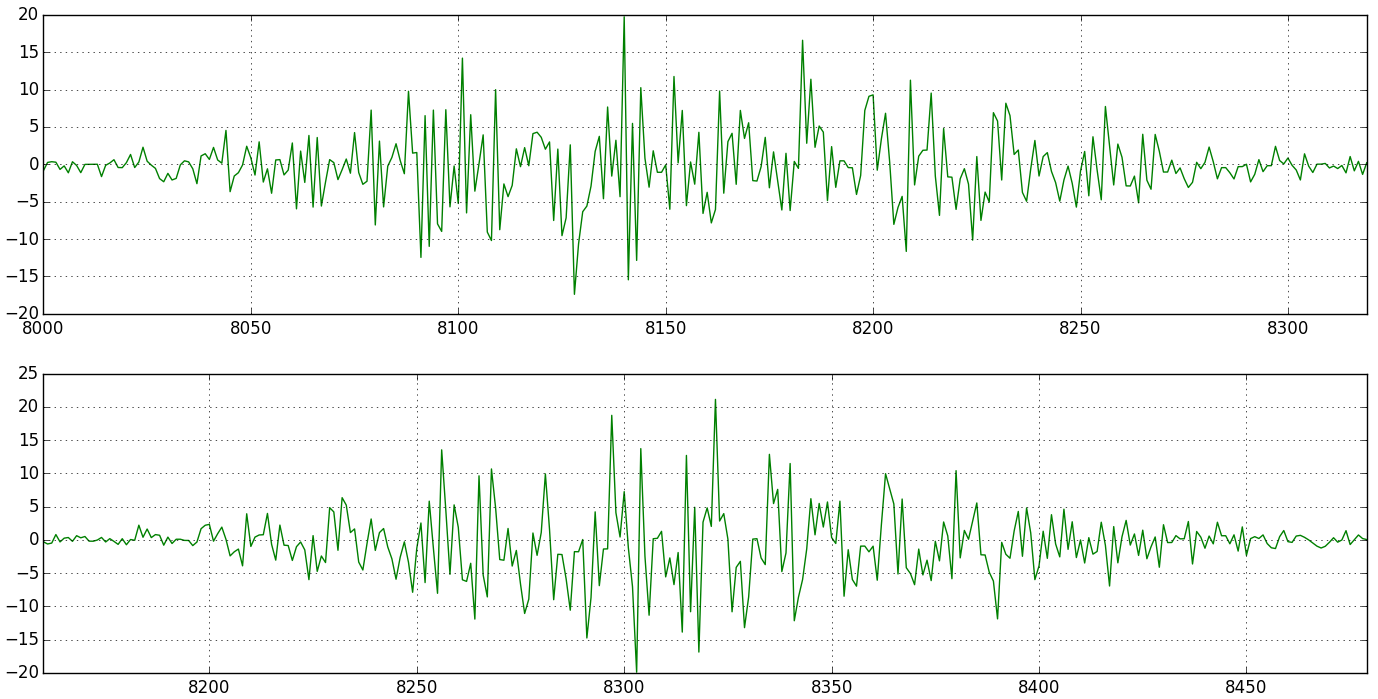
\includegraphics[width=0.75\textwidth]{framing}
\end{figure}
\end{frame}

\subsection{MFCC - Extração}

\begin{frame}
\frametitle{MFCC - Extração}
\begin{figure}[ht]
    \centering
    
\includegraphics[width=0.75\textwidth]{mfcc-flow}
\end{figure}
\pause

\begin{description}
    \item[$|FFT|^2$] Calcula o \textbf{espectro de potência}
    \pause
\end{description}
\begin{figure}[ht]
    \centering
    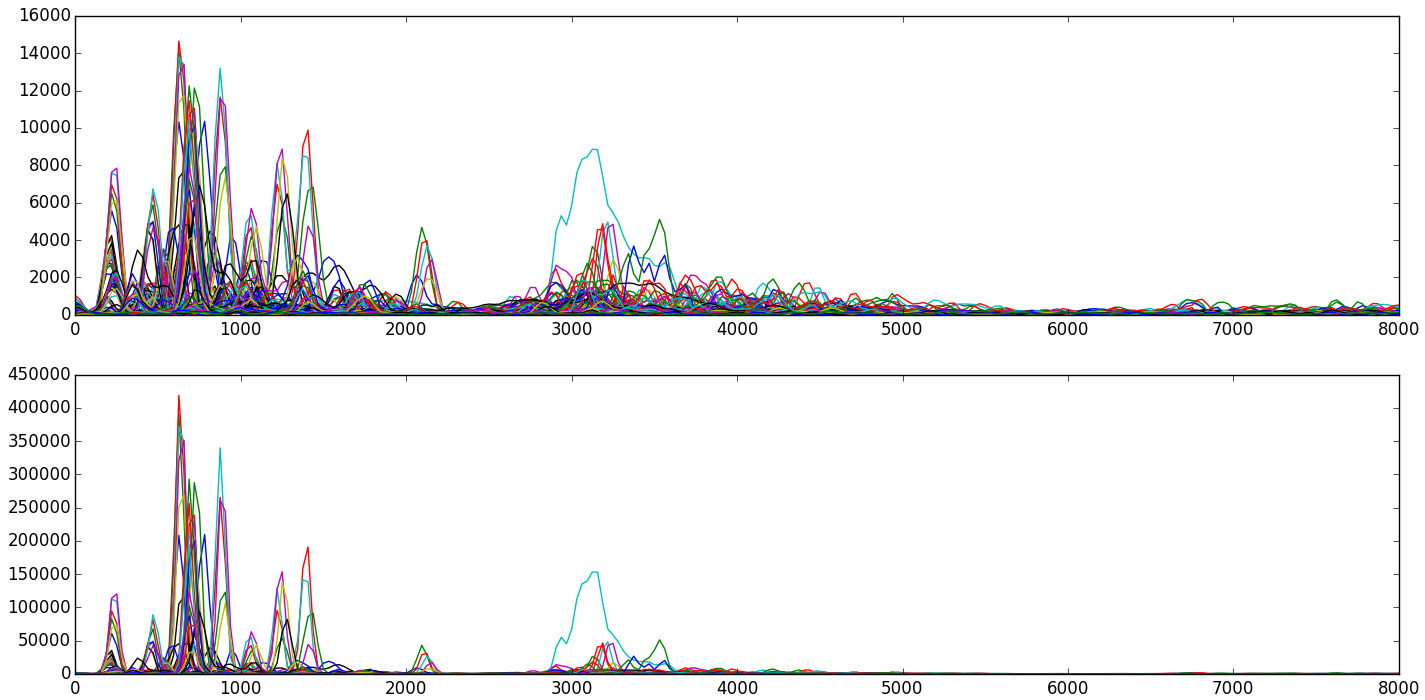
\includegraphics[width=0.6\textwidth]{fft}
\end{figure}
\end{frame}

\subsection{MFCC - Extração}

\begin{frame}
\frametitle{MFCC - Extração}
\begin{figure}[ht]
    \centering
    
\includegraphics[width=0.75\textwidth]{mfcc-flow}
\end{figure}
\pause

\begin{description}
    \item[Filtros] Espectro em Hz $\implies$ espectro em \textbf{mels}
    \pause
\end{description}
\begin{figure}[ht]
    \centering
    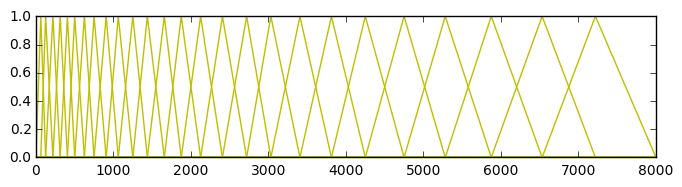
\includegraphics[width=0.75\textwidth]{filterbank}
\end{figure}
\end{frame}

\subsection{MFCC - Extração}

\begin{frame}
\frametitle{MFCC - Extração}
\begin{figure}[ht]
    \centering
    
\includegraphics[width=0.75\textwidth]{mfcc-flow}
\end{figure}
\pause

\begin{description}
    \item[dB] Calcula a \textbf{sonoridade}
    \pause
\end{description}
\begin{figure}[ht]
    \centering
    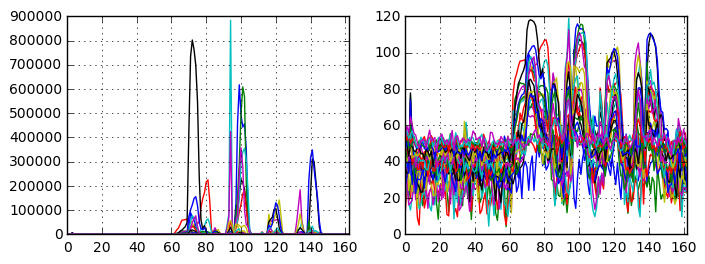
\includegraphics[width=0.75\textwidth]{features_and_featuresdB}
\end{figure}
\end{frame}

\subsection{MFCC - Extração}

\begin{frame}
\frametitle{MFCC - Extração}
\begin{figure}[ht]
    \centering
    
\includegraphics[width=0.75\textwidth]{mfcc-flow}
\end{figure}
\pause

\begin{description}
    \item[DCT] Coeficientes espectrais $\implies$ coeficientes \textbf{cepstrais}
    \pause
    \begin{itemize}
        \item $c_n = \sum_{k=1}^K S_k\cdot\cos\left[n\left(k - \frac{1}{2}\right)\frac{\pi}{K}\right], n = 1, 2, ..., L$
        \pause
    \end{itemize}
\end{description}
\begin{figure}[ht]
    \centering
    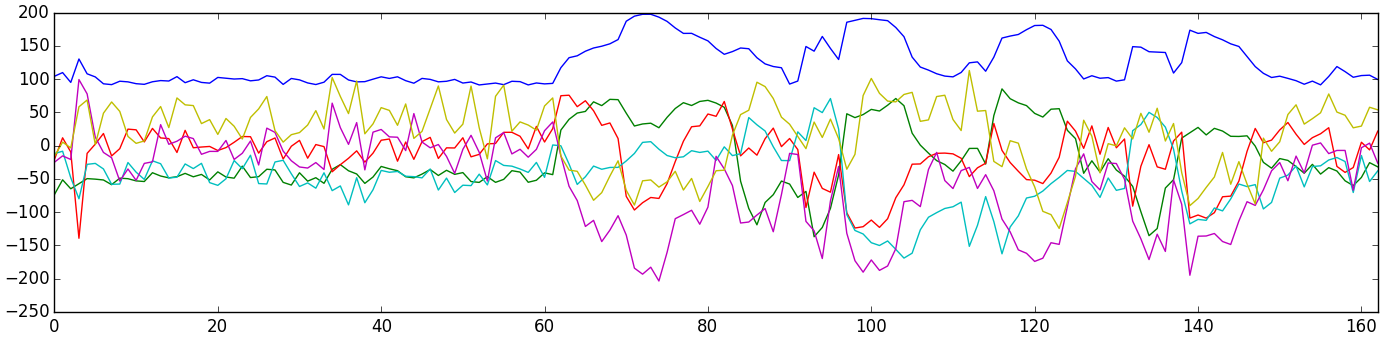
\includegraphics[width=0.7\textwidth]{mfcc}
\end{figure}
\begin{figure}[ht]
    \centering
    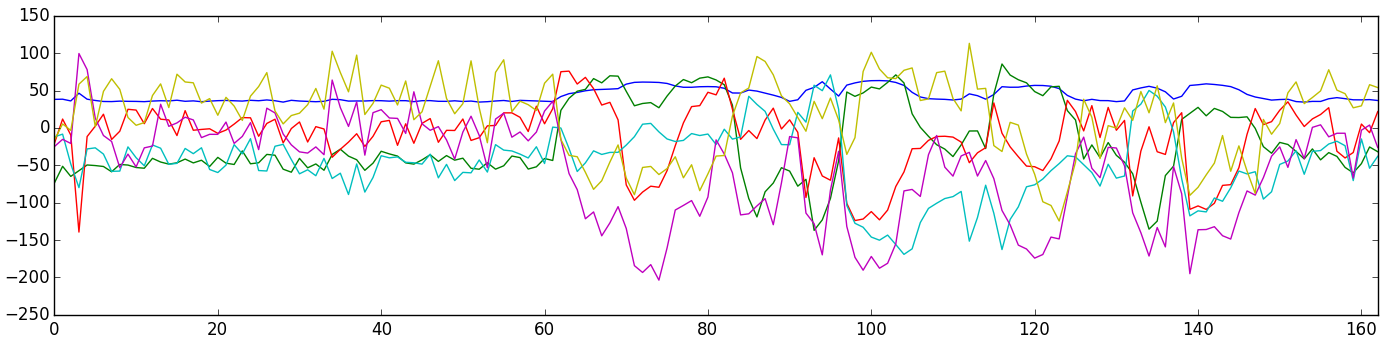
\includegraphics[width=0.7\textwidth]{mfcc_energy_appended}
\end{figure}
\end{frame}

\subsection{MFCC - Extração}

\begin{frame}
\frametitle{MFCC - Extração}
\begin{figure}[ht]
    \centering
    
\includegraphics[width=0.75\textwidth]{mfcc-flow}
\end{figure}
\pause

\begin{description}
    \item[CMS] \textbf{Normaliza} os MFCCs para reduzir perturbações
    \pause
    \begin{itemize}
        \item $c_n = c_n - \frac{1}{T} \sum_{t=1}^T c_{n,t}$
        \pause
    \end{itemize}
\end{description}
\begin{figure}[ht]
    \centering
    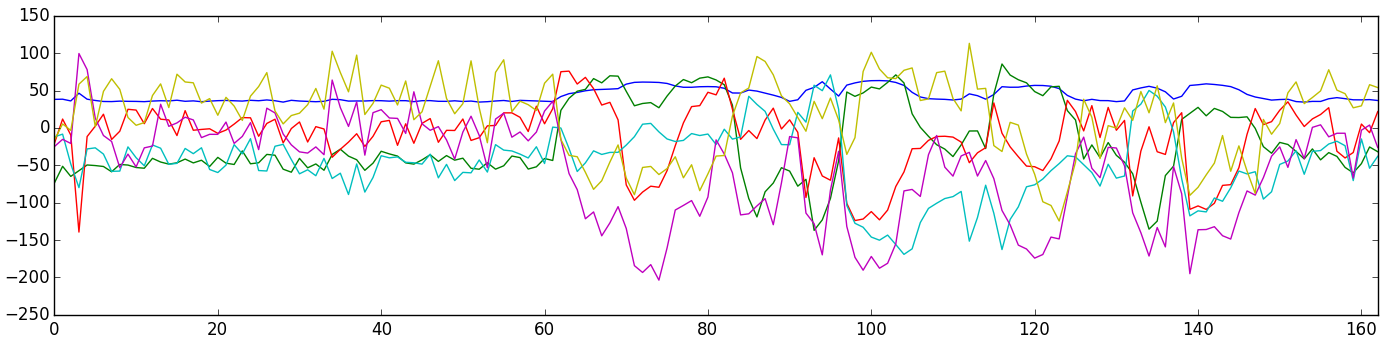
\includegraphics[width=0.7\textwidth]{mfcc_energy_appended}
\end{figure}
\begin{figure}[ht]
    \centering
    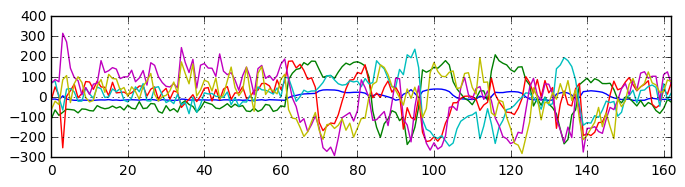
\includegraphics[width=0.7\textwidth]{mfcc_energy_appended_cms}
\end{figure}
\end{frame}

\subsection{MFCC - Extração}

\begin{frame}
\frametitle{MFCC - Extração}
\begin{figure}[ht]
    \centering
    
\includegraphics[width=0.75\textwidth]{mfcc-flow}
\end{figure}
\pause

\begin{description}
    \item[$\dvec{\Delta}$s] Novos $c_n$ \textbf{derivados} dos antigos $c_n$ (opcional)
    \pause
    \begin{itemize}
        \item $\Delta_t = \frac{\sum_{n=1}^N n(c_{t+n} - c_{t-n})}{2\sum_{n=1}^N n^2}$
        \pause
    \end{itemize}
\end{description}
\begin{figure}[ht]
    \centering
    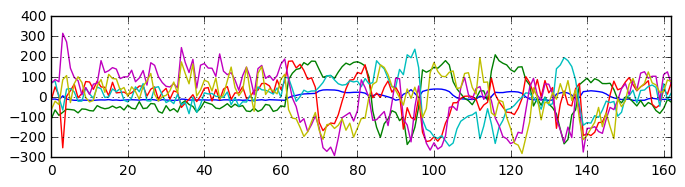
\includegraphics[width=0.7\textwidth]{mfcc_energy_appended_cms}
\end{figure}
\begin{figure}[ht]
    \centering
    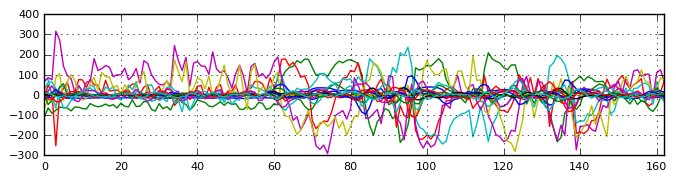
\includegraphics[width=0.7\textwidth]{mfcc_energy_appended_cms_delta_order_2}
\end{figure}
\end{frame}


% Backmatter

%\appendix
%
%
%\nocite{*}
%\bibliographystyle{alpha}
%\bibliography{biblio}

\end{document}